%% Requires compilation with XeLaTeX or LuaLaTeX
\documentclass[10pt,xcolor={table,dvipsnames},t]{beamer}
\usetheme{UCBerkeley}
\usepackage{tikz}
\usepackage{graphicx}
\usepackage{amsmath,amsthm,amssymb}
\usepackage{float}
\usepackage{comment}
\usepackage{tikz-cd}
\usepackage{setspace}
\usepackage{makecell}

\title[Your Short Title]{From Quasars to Quarks: Day 2.1}
\subtitle{Special Relativity}
\author{Charlie Cummings \& Shaunak Modak}
\institute{tinyurl.com/FQ2Q-relativity}
\date{September 9, 2020}

\begin{document}

\begin{frame}
    \titlepage
\end{frame}

% Uncomment these lines for an automatically generated outline.
\begin{frame}{Outline}
    \tableofcontents
\end{frame}

\section{Events and Geometry}
%softer stuff will be mostly bullets and pics, little drawing
\begin{frame}{Recap of Lagrangian Mechanics}
    \begin{enumerate}
        \item Inertial frames exist
        \item The true path makes the action $S = \int L dt$ stationary
        \item Space is homogeneous (and isotropic)
    \end{enumerate}
\end{frame}

\begin{frame}{Space and Coordinates}
\begin{itemize}
    \item What is space?
    % where things happen
    \item What are coordinates?
    %the numbers we give to spatial positions
    \item What's the difference?
\end{itemize}
\end{frame}

\begin{frame}{Events}
\begin{itemize}
    \item In general, we need \textbf{four} numbers to tell you where to find something: $(t,x,y,z)$ for example
    \item ``Position'' should be \textbf{four dimensional}
    \item How does this relate to how we normally think of space and time?
\end{itemize}
    
\end{frame}

\begin{frame}{Events and Coordinates}
\vfill
\begin{figure}[H]
    \centering
    \begin{tikzpicture}
        \draw[<->] (-5,0) -- (5,0);
        \filldraw[red] (0,0) circle (2pt);
        \draw (5.25,0) node{\textit{x}};
    \end{tikzpicture}
    \label{fig:1D}
\end{figure}
%need space for existence
%need time for dynamics
\end{frame}

\begin{frame}{Events and Coordinates}
\begin{figure}[H]
    \centering
    \begin{tikzpicture}[scale=0.75]
        \draw[<->] (-5,0) -- (5,0);
        \draw[<->] (0,-1) -- (0,5);
        \filldraw[red] (0,0) circle (2pt);
        \draw (5.25,0) node{\textit{x}};
        \draw (0,5.25) node{\textit{t}};
    \end{tikzpicture}
    \label{fig:1+1D}
\end{figure}
%draw the worldlines of: particle at x=0,1 for all t, particle with constant v, particle that turns around
%slope is 1/v
\end{frame}

%!!!!!!!!!!!! slide explaining t vs ct

\begin{frame}{The Principle of Relativity}

\begin{figure}[H]
    \centering
    \begin{tikzpicture}[scale=0.75]
        \draw[<->] (-5,0) -- (5,0);
        \draw[<->] (0,-1) -- (0,5);
        \draw[->, thick, blue] (0,0) -- (4,5);
        \draw[->, thick, red] (0,0) -- (0,5);
        
        \draw (5.25,0) node{\textit{x}};
        \draw (0,5.25) node{\textit{ct}};
    \end{tikzpicture}
    \label{fig:1+1D_wl}
\end{figure}
    
\end{frame}

\begin{frame}{The Principle of Relativity}

\begin{figure}[H]
    \centering
    \begin{tikzpicture}[scale=0.75]
        \draw[<->] (-5,0) -- (5,0);
        \draw[<->] (0,-1) -- (0,5);
        \draw[->, thick, blue] (0,0) -- (0,5);
        \draw[->, thick, red] (0,0) -- (-4,5);
        
        \draw (5.25,0) node{\textit{x}};
        \draw (0,5.25) node{\textit{ct}};
    \end{tikzpicture}
    \label{fig:1+1D_wl}
\end{figure}
    
\end{frame}

\begin{frame}{The Principle of Relativity}

\begin{figure}[H]
    \centering
    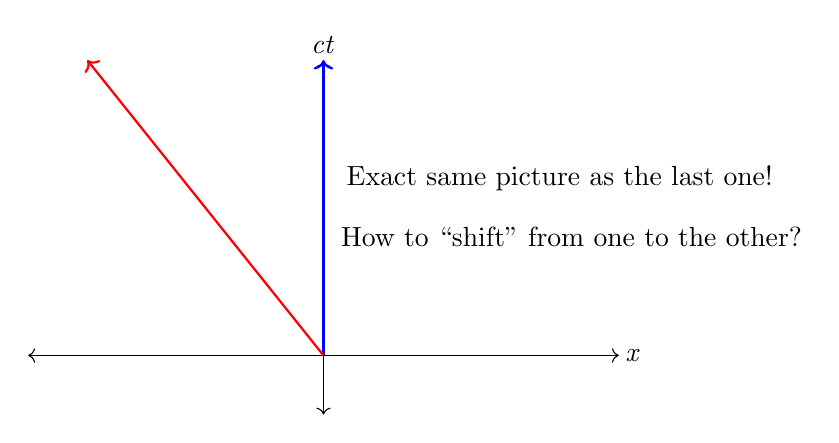
\begin{tikzpicture}[scale=0.75]
        \draw[<->] (-5,0) -- (5,0);
        \draw[<->] (0,-1) -- (0,5);
        \draw[->, thick, blue] (0,0) -- (0,5);
        \draw[->, thick, red] (0,0) -- (-4,5);
        
        \draw (5.25,0) node{\textit{x}};
        \draw (0,5.25) node{\textit{ct}};
        \node at (4,3) {Exact same picture as the last one!};
        \node at (4.2,2) {How to ``shift'' from one to the other?};
    \end{tikzpicture}
    \label{fig:1+1D_wl}
\end{figure}
    
\end{frame}

\begin{frame}{Galilean Transformations?}

\begin{figure}[H]
    \centering
    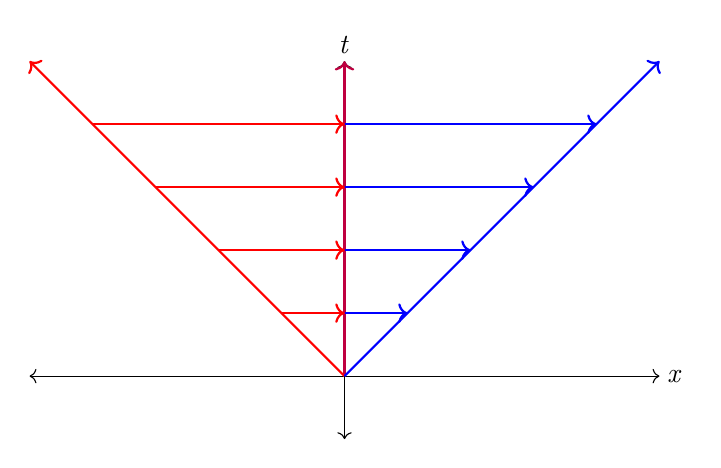
\begin{tikzpicture}[scale=0.8]
        \draw[<->] (-5,0) -- (5,0);
        \draw[<->] (0,-1) -- (0,5);
        \draw[->, thick, purple] (0,0) -- (0,5);
        \draw[->, thick, red] (0,0) -- (-5,5);
        \draw[->, thick, blue] (0,0) -- (5,5);
        
        \draw[->, thick, red] (-1,1) -- (0,1);
        \draw[->, thick, red] (-2,2) -- (0,2);
        \draw[->, thick, red] (-3,3) -- (0,3);
        \draw[->, thick, red] (-4,4) -- (0,4);
        
        \draw[->, thick, blue] (0,1) -- (1,1);
        \draw[->, thick, blue] (0,2) -- (2,2);
        \draw[->, thick, blue] (0,3) -- (3,3);
        \draw[->, thick, blue] (0,4) -- (4,4);
        
        \draw (5.25,0) node{\textit{x}};
        \draw (0,5.25) node{\textit{t}};
    \end{tikzpicture}
\end{figure}
    
\end{frame}

\begin{frame}{An Extra Assumption}
    \begin{itemize}
        \item Light has the same speed in all reference frames
        \item Required by Maxwell's Equations and proved by the Michelson Morley Experiment
    \end{itemize}
\end{frame}

\begin{frame}{An Extra Assumption}
    \begin{itemize}
        \item Light has the same speed in all reference frames
        \item Required by Maxwell's Equations and proved by the Michelson Morley Experiment
        \item Information has a (finite) maximum speed
        \item Time is different than space
    \end{itemize}
\end{frame}

\begin{frame}{Stretching and Shrinking}
    \begin{figure}[H]
    \centering
    \begin{tikzpicture}[scale=0.8]
        \def\pt{2}
        \draw[<->] (-5,0) -- (5,0);
        \draw[<->] (0,-1) -- (0,5);
        \draw[->,dashed] (0,0) -- (5,5);
        \draw[->,dashed] (0,0) -- (-5,5);
        
        \draw[->,red] (0,0) -- ({sinh(\pt)},{cosh(\pt)});
        
        \draw[red,dashed] plot[smooth,domain=\pt:2] ({sinh(\x)},{cosh(\x)});

        \draw (5.25,0) node{\textit{x}};
        \draw (0,5.25) node{\textit{t}};
    \end{tikzpicture}
\end{figure}
\end{frame}

\begin{frame}{Stretching and Shrinking}
    \begin{figure}[H]
    \centering
    \begin{tikzpicture}[scale=0.8]
        \def\pt{1}
        \draw[<->] (-5,0) -- (5,0);
        \draw[<->] (0,-1) -- (0,5);
        \draw[->,dashed] (0,0) -- (5,5);
        \draw[->,dashed] (0,0) -- (-5,5);
        
        \draw[->,red] (0,0) -- ({sinh(\pt)},{cosh(\pt)});
        
        \draw[red,dashed] plot[smooth,domain=\pt:2] ({sinh(\x)},{cosh(\x)});

        \draw (5.25,0) node{\textit{x}};
        \draw (0,5.25) node{\textit{t}};
    \end{tikzpicture}
\end{figure}
\end{frame}

\begin{frame}{Stretching and Shrinking}
    \begin{figure}[H]
    \centering
    \begin{tikzpicture}[scale=0.8]
        \def\pt{0}
        \draw[<->] (-5,0) -- (5,0);
        \draw[<->] (0,-1) -- (0,5);
        \draw[->,dashed] (0,0) -- (5,5);
        \draw[->,dashed] (0,0) -- (-5,5);
        
        \draw[->,red] (0,0) -- ({sinh(\pt)},{cosh(\pt)});
        
        \draw[red,dashed] plot[smooth,domain=\pt:2] ({sinh(\x)},{cosh(\x)});

        \draw (5.25,0) node{\textit{x}};
        \draw (0,5.25) node{\textit{t}};
    \end{tikzpicture}
\end{figure}
\end{frame}

\begin{frame}{Stretching and Shrinking}
    \begin{figure}[H]
    \centering
    \begin{tikzpicture}[scale=0.8]
        \def\pt{-1}
        \draw[<->] (-5,0) -- (5,0);
        \draw[<->] (0,-1) -- (0,5);
        \draw[->,dashed] (0,0) -- (5,5);
        \draw[->,dashed] (0,0) -- (-5,5);
        
        \draw[->,red] (0,0) -- ({sinh(\pt)},{cosh(\pt)});
        
        \draw[red,dashed] plot[smooth,domain=\pt:2] ({sinh(\x)},{cosh(\x)});

        \draw (5.25,0) node{\textit{x}};
        \draw (0,5.25) node{\textit{t}};
    \end{tikzpicture}
\end{figure}
\end{frame}

\begin{frame}{Stretching and Shrinking}
    \begin{figure}[H]
    \centering
    \begin{tikzpicture}[scale=0.8]
        \def\pt{-2}
        \draw[<->] (-5,0) -- (5,0);
        \draw[<->] (0,-1) -- (0,5);
        \draw[->,dashed] (0,0) -- (5,5);
        \draw[->,dashed] (0,0) -- (-5,5);
        
        \draw[->,red] (0,0) -- ({sinh(\pt)},{cosh(\pt)});
        
        \draw[red,dashed] plot[smooth,domain=\pt:2] ({sinh(\x)},{cosh(\x)});

        \draw (5.25,0) node{\textit{x}};
        \draw (0,5.25) node{\textit{t}};
    \end{tikzpicture}
\end{figure}
\end{frame}

\begin{frame}{The Same Idea}
    \begin{figure}[H]
    \centering
    \begin{tikzpicture}
        \def\pt{0}
        \draw[<->] (-2,0) -- (2,0);
        \draw[<->] (0,-2) -- (0,2);
        
        \draw[->,red] (0,0) -- ({cos(\pt)},{sin(\pt)});
        
        \draw[red,dashed] plot[smooth,domain=0:\pt] ({cos(\x)},{sin(\x)});

        \draw (2.25,0) node{\textit{x}};
        \draw (0,2.25) node{\textit{y}};
    \end{tikzpicture}
\end{figure}
\end{frame}

\begin{frame}{The Same Idea}
    \begin{figure}[H]
    \centering
    \begin{tikzpicture}
        \def\pt{45}
        \draw[<->] (-2,0) -- (2,0);
        \draw[<->] (0,-2) -- (0,2);
        
        \draw[->,red] (0,0) -- ({cos(\pt)},{sin(\pt)});
        
        \draw[red,dashed] plot[smooth,domain=0:\pt] ({cos(\x)},{sin(\x)});

        \draw (2.25,0) node{\textit{x}};
        \draw (0,2.25) node{\textit{y}};
    \end{tikzpicture}
\end{figure}
\end{frame}

\begin{frame}{The Same Idea}
    \begin{figure}[H]
    \centering
    \begin{tikzpicture}
        \def\pt{135}
        \draw[<->] (-2,0) -- (2,0);
        \draw[<->] (0,-2) -- (0,2);
        
        \draw[->,red] (0,0) -- ({cos(\pt)},{sin(\pt)});
        
        \draw[red,dashed] plot[smooth,domain=0:\pt] ({cos(\x)},{sin(\x)});

        \draw (2.25,0) node{\textit{x}};
        \draw (0,2.25) node{\textit{y}};
    \end{tikzpicture}
\end{figure}
\end{frame}

\begin{frame}{The Same Idea}
    \begin{figure}[H]
    \centering
    \begin{tikzpicture}
        \def\pt{275}
        \draw[<->] (-2,0) -- (2,0);
        \draw[<->] (0,-2) -- (0,2);
        
        \draw[->,red] (0,0) -- ({cos(\pt)},{sin(\pt)});
        
        \draw[red,dashed] plot[smooth,domain=0:\pt] ({cos(\x)},{sin(\x)});

        \draw (2.25,0) node{\textit{x}};
        \draw (0,2.25) node{\textit{y}};
    \end{tikzpicture}
\end{figure}
\end{frame}

\begin{frame}{Fundamental Shapes and Geometry}
    \begin{itemize}
        \item For the $x-y$ plane, the circle $r^2 = x^2+y^2$ is the fundamental shape
        \item For the $x-t$ plane, the hyperbola $\tau^2 = t^2-x^2$ is the fundamental shape
    \end{itemize}
\end{frame}

\begin{frame}{Fundamental Shapes and Geometry}
    \begin{itemize}
        \item For the $x-y$ plane, the circle $r^2 = x^2+y^2$ is the fundamental shape
        \item For the $x-t$ plane, the hyperbola $\tau^2 = t^2-x^2$ is the fundamental shape
        \item For the $x-y$ plane, the \textbf{metric} is $ds^2 = dx^2 + dy^2$
        \item For the $x-t$ plane, the \textbf{metric} is $d\tau^2 = dt^2 - dx^2$
    \end{itemize}
\end{frame}

\begin{frame}{Fundamental Shapes and Geometry}
    \begin{itemize}
        \item For all of spacetime, the \textbf{metric} is $d\tau^2 = dt^2 - dx^2 - dy^2 - dz^2$
    \end{itemize}
    
    \begin{equation*}
        \eta_{\mu \nu} = \begin{bmatrix}1 & 0 & 0 & 0 \\ 0 & -1 & 0 & 0 \\ 0 & 0 & -1 & 0 \\ 0 & 0 & 0 & -1 \end{bmatrix}
    \end{equation*}
\end{frame}

\begin{frame}{Time Dilation: $t = \gamma \tau$}
    \begin{figure}[H]
    \centering
    \begin{tikzpicture}[scale=0.8]
        \draw[<->] (-5,0) -- (5,0);
        \draw[<->] (0,-1) -- (0,5);
        \draw[dashed,->] (0,0) -- (5,5);
        \draw[dashed,->] (0,0) -- (-5,5);
        
        \draw[red,->] (0,0) -- ({sinh(0)},{cosh(0)});
        \draw[red,->] (0,0) -- ({sinh(0.5)},{cosh(0.5)});
        \draw[red,->] (0,0) -- ({sinh(1)},{cosh(1)});
        \draw[red,->] (0,0) -- ({sinh(1.5)},{cosh(1.5)});
        \draw[red,->] (0,0) -- ({sinh(2)},{cosh(2)});
        
        \draw (-0.1,{cosh(0)}) -- (0.1,{cosh(0)});
        \draw (-0.1,{cosh(0.5)}) -- (0.1,{cosh(0.5)});
        \draw (-0.1,{cosh(1)}) -- (0.1,{cosh(1)});
        \draw (-0.1,{cosh(1.5)}) -- (0.1,{cosh(1.5)});
        \draw (-0.1,{cosh(2)}) -- (0.1,{cosh(2)});
        
        \draw (5.25,0) node{\textit{x}};
        \draw (0,5.25) node{\textit{t}};
    \end{tikzpicture}
    \label{fig:1+1D_wl}
\end{figure}

\end{frame}

\begin{frame}{Length Contraction: $L' = \frac{L_0}{\gamma}$}
    \begin{figure}[H]
    \centering
    \begin{tikzpicture}[scale=0.8]
        \draw[<->] (-5,0) -- (5,0);
        \draw[<->] (0,-1) -- (0,5);
        
        \draw[red] plot[smooth,domain=-2:2] ({sinh(\x)},{cosh(\x)});
        \draw[blue] plot[smooth,domain=-2.71:2.71] ({0.5*sinh(\x)},{0.5*cosh(\x)});

        \draw (5.25,0) node{\textit{x}};
        \draw (0,5.25) node{\textit{t}};
    \end{tikzpicture}
    \label{fig:1+1D_wl}
\end{figure}

\end{frame}

\begin{frame}{Purely Geometrical Effects}
    \begin{itemize}
        \item While it is natural to ask for a mechanism, there is none
        \item What is the mechanism for ``x contraction'' or ``y dilation'' in rotations?
    \end{itemize}
\end{frame}

\begin{frame}{Breakout Question}
 A pole vaulter has a 5m long pole and a farmer has a 3m long barn. The pole vaulter bets the farmer they can fit the pole inside the barn all at once! Their plan is to run at a speed $\beta = \frac{4}{5}$ so that in the barn's rest frame, $L_{pole} = \frac{5m}{\gamma} = \frac{5m}{\frac{5}{3}} = 3m$. At the instant the the pole is fully inside the barn, the farmer quickly closes and opens the doors, so that the pole is ``inside the barn'' at that exact moment in time.
 
 \vspace{10pt}
 
 Problem: In the pole vaulter's frame, the barn is the one that's moving! The barn has length contracted in their frame to $L_{barn} = \frac{3m}{\frac{5}{3}} = 1.8m$. But the events of the front and back doors closing definitely happened, so what gives?


\end{frame}

\begin{frame}{Lorentz Transformations}
    \begin{align*}
        ct' = \gamma(ct - \frac{v}{c} x) \\
        x' = \gamma(x - \frac{v}{c} ct)
    \end{align*}
\end{frame}

\begin{frame}{Lorentz Transformations}
    \begin{align*}
        t' = \gamma(t - \beta x) \\
        x' = \gamma(x - \beta t)
    \end{align*}
    
    \begin{equation*}
        \begin{bmatrix}t' \\ x' \end{bmatrix} = \begin{bmatrix}\gamma & -\gamma \beta \\ -\gamma \beta & \gamma  \end{bmatrix} \begin{bmatrix}t \\ x \end{bmatrix}
    \end{equation*}
\end{frame}

\begin{frame}{Lorentz Transformations}
    \begin{align*}
        t' = \gamma(t - \beta x) \\
        x' = \gamma(x - \beta t)
    \end{align*}
    
    \begin{equation*}
        \begin{bmatrix}t' \\ x' \end{bmatrix} = \begin{bmatrix}\gamma & -\gamma \beta \\ -\gamma \beta & \gamma  \end{bmatrix} \begin{bmatrix}t \\ x \end{bmatrix}
    \end{equation*}
    \vspace{10pt}
    \begin{equation*}
        {\Lambda^\mu}_\nu = \begin{bmatrix}\gamma & -\gamma \beta \\ -\gamma \beta & \gamma  \end{bmatrix}
    \end{equation*}
\end{frame}

\begin{frame}{4-vectors}
    \begin{itemize}
        \item In index notation, we can write $x^j = \begin{bmatrix} x \\ y \\ z \end{bmatrix}$
        \item In index notation, we can write $x^\mu = \begin{bmatrix} t\\ x \\ y \\ z \end{bmatrix}$
        \item What are some other 4-vectors we can make?
    \end{itemize}
\end{frame}

\begin{frame}{Velocity vs Proper Velocity}
    \begin{itemize}
        \item Normally, $v^{\hspace{1pt}j} = \frac{d}{dt}x^{\hspace{1pt}j}$ but now $t = x^0$
        \item $\frac{dx'}{dt'} = \frac{dx-vdt}{dt-vdx} = \frac{dx/dt-v}{1-vdx/dt}$... gross
        \item Is there a more invariant notion of velocity?
    \end{itemize}
\end{frame}

\begin{frame}{Velocity vs Proper Velocity}
    \begin{itemize}
        \item $v^\mu = \frac{d}{dt}x^\mu = \begin{bmatrix} \frac{dt}{dt} \\ \frac{d\Vec{x}}{dt} \end{bmatrix} = \begin{bmatrix} 1 \\ \vec{v} \end{bmatrix}$
    \end{itemize}
\end{frame}

\begin{frame}{Velocity vs Proper Velocity}
    \begin{itemize}
        \item $v^\mu = \frac{dx^\mu}{dt} = \begin{bmatrix} \frac{dt}{dt} \\ \frac{d\Vec{x}}{dt} \end{bmatrix} = \begin{bmatrix} 1 \\ \vec{v} \end{bmatrix}$
        \item $u^\mu = \frac{dx^\mu}{d\tau} = \begin{bmatrix} \frac{dt}{d\tau} \\ \frac{d\Vec{x}}{dt}\frac{dt}{d\tau} \end{bmatrix} = \begin{bmatrix} \gamma \\ \gamma \vec{v} \end{bmatrix} = \gamma v^\mu$
        %show |u|=1
    \end{itemize}
\end{frame}

\section{Energy and Momentum}

\begin{frame}{4-Momentum}
    \begin{itemize}
        \item $p^\mu = m u^\mu = \begin{bmatrix} m\gamma \\ m\gamma \vec{v} \end{bmatrix}$
    \end{itemize}
\end{frame}

\begin{frame}{4-Momentum}
    \begin{itemize}
        \item $p^\mu = m u^\mu = \begin{bmatrix} m\gamma \\ m\gamma \vec{v} \end{bmatrix}$
        \item What is $p^0 = m\gamma$?
    \end{itemize}
\end{frame}

\begin{frame}{4-Momentum}
    \begin{itemize}
        \item $p^\mu = m u^\mu = \begin{bmatrix} m\gamma \\ m\gamma \vec{v} \end{bmatrix}$
        \item What is $p^0 = \frac{mc}{\left(1-\frac{v^2}{c^2}\right)^{\frac{1}{2}}}$?
        \item Taylor expand: $p^0c \approx mc^2(1+\frac{1}{2}\frac{v^2}{c^2}) = mc^2 + \frac{1}{2}mv^2$
        \item It's the energy!
        % p^2=m^2?
    \end{itemize}
\end{frame}

\section{Takeaways}

\begin{frame}{The Action Revisited}
    \begin{itemize}
        \item Lagrangian is $L = K-U = p_j \dot{q}^j - H$
        \item The differential for the action is $dS = Ldt$
        \item $Ldt = p_j \dot{q}^jdt - Hdt = p_j dq^j - Hdt = -p_\mu dq^\mu$
        \item Chain rule: $dS = -mu_\mu \frac{dq^\mu}{d\tau}d\tau = -m(u_\mu u^\mu) d\tau = -md\tau$
        \item Stationary action $\iff$ Worldlines are ``geodesics'' through spacetime
    \end{itemize}
\end{frame}

\begin{frame}{Recap of Lagrangian Mechanics in Special Relativity}
    \begin{enumerate}
        \item Particles travel along geodesics (straightest possible lines)
        \item Space is homogeneous (and isotropic)
    \end{enumerate}
    \vfill
\begin{figure}
    \centering
    \def\omu{26}
    \def\oml{-30}
    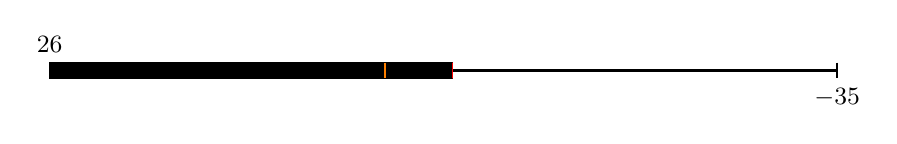
\begin{tikzpicture}
    
    %labels
    \node[anchor=south] at (-5,0.1) {\small $26$};
    \node[anchor=south] at (-0.1639*\omu-0.7377,0.1) {\small $\omu$};
    \node[anchor=north] at (-0.1639*\oml-0.7377,-0.1) {\small $\oml$};
    \node[anchor=north] at (5,-0.1) {\small $-35$};
    
    %blue fill bar
    \filldraw (-5,0.1) -- (-0.1639*\omu-0.7377,0.1) -- (-0.1639*\omu-0.7377,-0.1) -- (-5,-0.1) -- cycle;
    %red fill bar
    \filldraw[red] (-0.1639*\omu-0.7377,-0.1) --  (-0.1639*\omu-0.7377,0.1) -- (-0.1639*\oml-0.7377,0.1)--(-0.1639*\oml-0.7377,-0.1) -- cycle;
    %blue thin bar
    \draw[thick] (-0.1639*\oml-0.731,0) -- (5,0);
    %vertical blue thin bar
    \draw[thick] (5,.1) -- (5,-.1);
    \draw[thick] (-5,.1) -- (-5,-.1);
    %1m mark
    \draw[thick, orange] (-0.7377,.1) -- (-0.7377,-.1);

    \end{tikzpicture}
    \label{fig:progress}
\end{figure}

\end{frame}



\end{document}
